\documentclass[12pt]{report}
\usepackage{../mystyle}
\usepackage{./slashbox}

\begin{document}
\newcommand{\HRule}{\rule{\linewidth}{0.5mm}}

\begin{titlepage}

\centering
	
\includegraphics[width=0.2\textwidth]{./title/logohse.png}\par\vspace{1cm}
	{\scshape \LARGE Higher School of Economics \\ \small(National Research University)\par}
	{\scshape \Large Faculty of Computer Science\par}
	\vspace{3cm}
	{\scshape\Large Home Assignment \par \Large{Course: ``Modern Methods of Data Analysis''}\par}
%	\vspace{1cm}
    \HRule \\[0.5cm]
    { \Large \bfseries Medium Articles Analysis}\\[0.2cm] % Title of your document
    \HRule
	\vspace{3.5cm}
	\begin{flushright}
	Student: Ryabykin Alexey \\
	Professor: Ignatov Dmitriy Igorevich
	\\
	Grade: \underline{\hspace{0.2cm}}
    \end{flushright}
    \vfill

	{\large Moscow, 2022}
\end{titlepage}
\boldmath
\tableofcontents
\newpage
\pagestyle{fancy}

\fancyhead[L]{Домашнее задание 2}
\fancyhead[C]{\currentname}
\fancyhead[R]{Рябыкин Алексей}

\section{Постановка задачи}
\par 
\emph{Выбранные данные:} Российский мониторинг экономического положения и здоровья населения НИУ ВШЭ (\href{https://www.hse.ru/rlms/spss}{RLMS-HSE}).
\par
Этапы работы:
\begin{enumerate*}
    \item Произвести отбор признаков для последующей классификации объектов с целью разделения общей совокупности на однородные подсовокупности. Произвести предварительный анализ этих признаков. Построить ортогональный базис из отобранных признаков методом главных компонент. Проанализировать возможность снижения размерности признакового пространства при сохранении в достаточной мере его информативности.
    \item Произвести параметрическую классификацию объектов в отсутствие обучения методом расщепления смесей вероятностных распределений по предполагаемому наиболее информативному признаку либо по первой главной компоненте; 
    \item Разбить объекты на кластеры в пространстве главных компонент. Сравнить результаты кластеризации и классификации на основе декомпозиции смеси распределений;
    \item Создать обучающую выборку из наиболее типичных представителей выделенных однородных групп объектов. Произвести классификацию объектов методом дискриминантного анализа. Произвести проверку правильности классификации методом кросс-валидации;
    \item Построить в выделенных одним из способов однородных группах регрессионные модели по иным, чем используемые в классификации, признакам. Сравнить полученные модели и сделать выводы по проделанной работе.
\end{enumerate*}
\par
\emph{Целью исследования} можно назвать формирование понимания и формализацию закономерностей в финансовой и имущественной обеспеченности населения России.
\par 
\emph{Регионом исследования} был выбран Москва.
\newpage
\section{Описание данных и выбранных признаков}
\par
\textcolor{red}{Повтор из прошлой работы}
\par
Доходы, исходя из данных и международных принципов их дифференциации, могут быть представлены следующими видами:
\begin{table}[H]
    \centering
    \begin{tabular}{|l|l|}
        \hline
        Доходы                                                  & Виды доходов в исследовании            \\ \hline
        \multicolumn{1}{|c|}{\multirow{4}{*}{Первичные доходы}} & Оплата труда                           \\ \cline{2-2} 
        \multicolumn{1}{|c|}{}                                  & Продажа сельскохозяйственной продукции \\ \cline{2-2} 
        \multicolumn{1}{|c|}{}                                  & Личное хозяйство                       \\ \cline{2-2} 
        \multicolumn{1}{|c|}{}                                  & Предпринимательская деятельность       \\ \hline
        \multirow{2}{*}{Собственность}                          & Аренда недвижимости                    \\ \cline{2-2} 
                                                                & Проценты                               \\ \hline
        \multirow{6}{*}{Трансферты}                             & Пенсии                                 \\ \cline{2-2} 
                                                                & Стипендии                              \\ \cline{2-2} 
                                                                & Пособия                                \\ \cline{2-2} 
                                                                & Алименты                               \\ \cline{2-2} 
                                                                & Пособия по безработице                 \\ \cline{2-2} 
                                                                & Другие доходы                          \\ \hline
        \multirow{2}{*}{Прочие поступления}                     & Продажа личного имущества              \\ \cline{2-2} 
                                                                & Продажа недвижимости                   \\ \hline
        \end{tabular}
\caption{Доходы и их виды}
\end{table}
\par
С другой стороны, среди расходов и имуществ населения можно выделить следующие группы для анализа:

\begin{table}[H]
    \parbox{0.45\linewidth}{\begin{tabular}{|l|l|}
    \hline
    Расходы                 & Примеры                     \\ \hline
    Потребительские расходы & Продукты питания            \\ \hline
    Платежи и взносы        & Налоги, связь, интернет     \\ \hline
    Приобретение имущества  & Квартиры, гараж и прочее    \\ \hline
    Денежные сбережения     & Вклады, сбережения в валюте \\ \hline
    \end{tabular}
    \caption{Расходы и их виды}
    } \hspace*{2cm}
       \parbox{0.45\linewidth}{\begin{tabular}{|l|l|}
        \hline
        Активы            & Примеры                \\ \hline
        Реальные активы   & Квартира, дача, машина \\ \hline
        Оборотные активы  & Одежда, наличные       \\ \hline
        Финансовые активы & Арендное имущество     \\ \hline
        \end{tabular}
        \caption{Типы имущества}
        }
\end{table}
Для решения поставленных задач были выбраны немного отличные от предыдущего домашнего задания данные.

\section{Предварительный анализ данных}
Выбранные данные содержат результаты опроса 413 респондентов из Москвы по практически 1.5 тысячам вопросам различного характера. 
\begin{longtable}{llcl}
  \toprule
   Столбец &                                                                                             Описание &  Количество п. з. & Доля п. з. \\
  \midrule
  \endfirsthead
  
  \toprule
   Столбец &                                                                                             Описание &  Количество п. з. & Доля п. з. \\
  \midrule
  \endhead
  \midrule
  \multicolumn{4}{r}{{Продолжение на следующей странице }} \\
  \midrule
  \endfoot
  
  \bottomrule
  \endlastfoot
  ze13.31b &       Траты на медикаменты &                               85 &                     20.6\% \\
  ze13.32b & Траты на моющие средства &                              113 &                     27.4\% \\
  ze13.33b & Траты на хоз товары &                               86 &                     20.8\% \\
    ze9.9b & Траты на интернет &                               63 &                     15.3\% \\
    ze9.8b &                        Траты на мобильную связь &                               13 &                      3.1\% \\
     zc1.1 &                                  Стоимость жильзя &                               10 &                      2.4\% \\
     zb1.o &                                          Численность домохозяйств &                               30 &                      7.3\% \\
       zc6 & Полезная площадь жилья &                                0 &                      0.0\% \\
       zc5 & Жилая площадь &                                0 &                      0.0\% \\
    zf12\_a & Как долго смогли бы жить только за счет сбережений?  &                                0 &                      0.0\% \\
  \end{longtable}
  Эта таблица может отличать от соответствующей в прошлом задании, потому что я обозначил все значения из множества $[$``ЗАТРУДНЯЮСЬ ОТВЕТИТЬ'', ``ЖИЛЬЕ ПРОДАТЬ НЕВОЗМОЖНО'', ``ЖИЛЬЕ НЕ ПОДЛЕЖИТ ПРОДАЖЕ'', ``ОТКАЗ ОТ ОТВЕТА'', ``НЕТ ОТВЕТА''$]$ за пропуски, чего не сделал в прошлый раз. Считаю так более репрентативно. Для столбцов траты на интернет, пропуски были заполнены нулями, для остальных средним и модой для количественных и качественного признаков, соответсвенно.
    \begin{note}{}
      Описание некоторых столбцов здесь и впредь было изменено для адекватного отображения таблиц, рисунков, диаграмм.
    \end{note}  
  \par
  Проведем предварительный анализ выбранных количественных признаков, рассчитав для каждого выборочные характеристики центральной тенденции и разброса:
    \par
\begin{table}[H]
  \centering
  \begin{tabular}{lrrrrrrr}
    \toprule
    {} &        mean &         std &        min &         25\% &         50\% &         75\% &         max \\
    \midrule
    Траты на медикаменты       &     2429.48 &     3134.18 &        0.0 &      410.00 &     1500.00 &     3000.00 &     30000.0 \\
    Траты на моющие средства &      647.68 &      528.08 &       30.0 &      380.00 &      647.47 &      647.47 &      5000.0 \\
    Траты на хоз товары &      749.06 &      872.78 &       40.0 &      350.00 &      647.47 &      800.00 &     10000.0 \\
    Траты на интернет                                       &      615.45 &      276.38 &        0.0 &      490.00 &      550.00 &      614.89 &      2000.0 \\
    Траты на мобильную связь                         &     1199.62 &     1273.79 &        0.0 &      500.00 &     1000.00 &     1500.00 &     20000.0 \\
    Стоимость жилья                                  &  9478285.7 &  3941801.8 &  2000000 &  6750000 &  9486781.61 &  12000000 &  20000000 \\
    Численность домохозяйств                                          &        2.55 &        1.44 &        1.0 &        1.00 &        2.00 &        3.00 &         9.0 \\
    Полезная площадь &       53.28 &       15.32 &       16.5 &       42.60 &       52.30 &       60.20 &       113.0 \\
    Жилая площадь &       34.11 &       12.16 &       11.0 &       26.55 &       32.00 &       42.00 &        77.0 \\
    Денежный доход                                                                                       &    88784.06 &    65912.56 &     4000.0 &    45000.00 &    70172.00 &   113500.00 &    631000.0 \\
    Траты на питание &    23377.69 &    12675.36 &     3500.0 &    15000.00 &    20000.00 &    30000.00 &    100000.0 \\
    \bottomrule
    \end{tabular}
\end{table}
\par 
Ниже приведены распределения и диаграммы рассеивания для выбранных для факторного анализа признаков:
\begin{table}[H]
  \centering
  \begin{tabular}{|c|c|}
  \hline
  Столбец  & Описание                         \\ \hline
  ze13.31b & Траты на медикаменты             \\ \hline
  ze13.32b & Траты на моющие средства         \\ \hline
  ze13.33b & Траты на средства личной гигиены \\ \hline
  ze9.9b   & Траты на Интернет                \\ \hline
  ze9.8b   & Траты на мобильную связь         \\ \hline
  ze11 & \begin{tabular}[c]{@{}c@{}}Траты на квартиру\\ (аренда, коммунальные услуги)\end{tabular} \\ \hline
  ze4  & \begin{tabular}[c]{@{}c@{}}Траты на питание\\ (дома и вне дома)\end{tabular}              \\ \hline
  \end{tabular}
  \caption{Выбранные для факторного анализа столбцы}
  \end{table}
\begin{figure}[H]
    \centering
    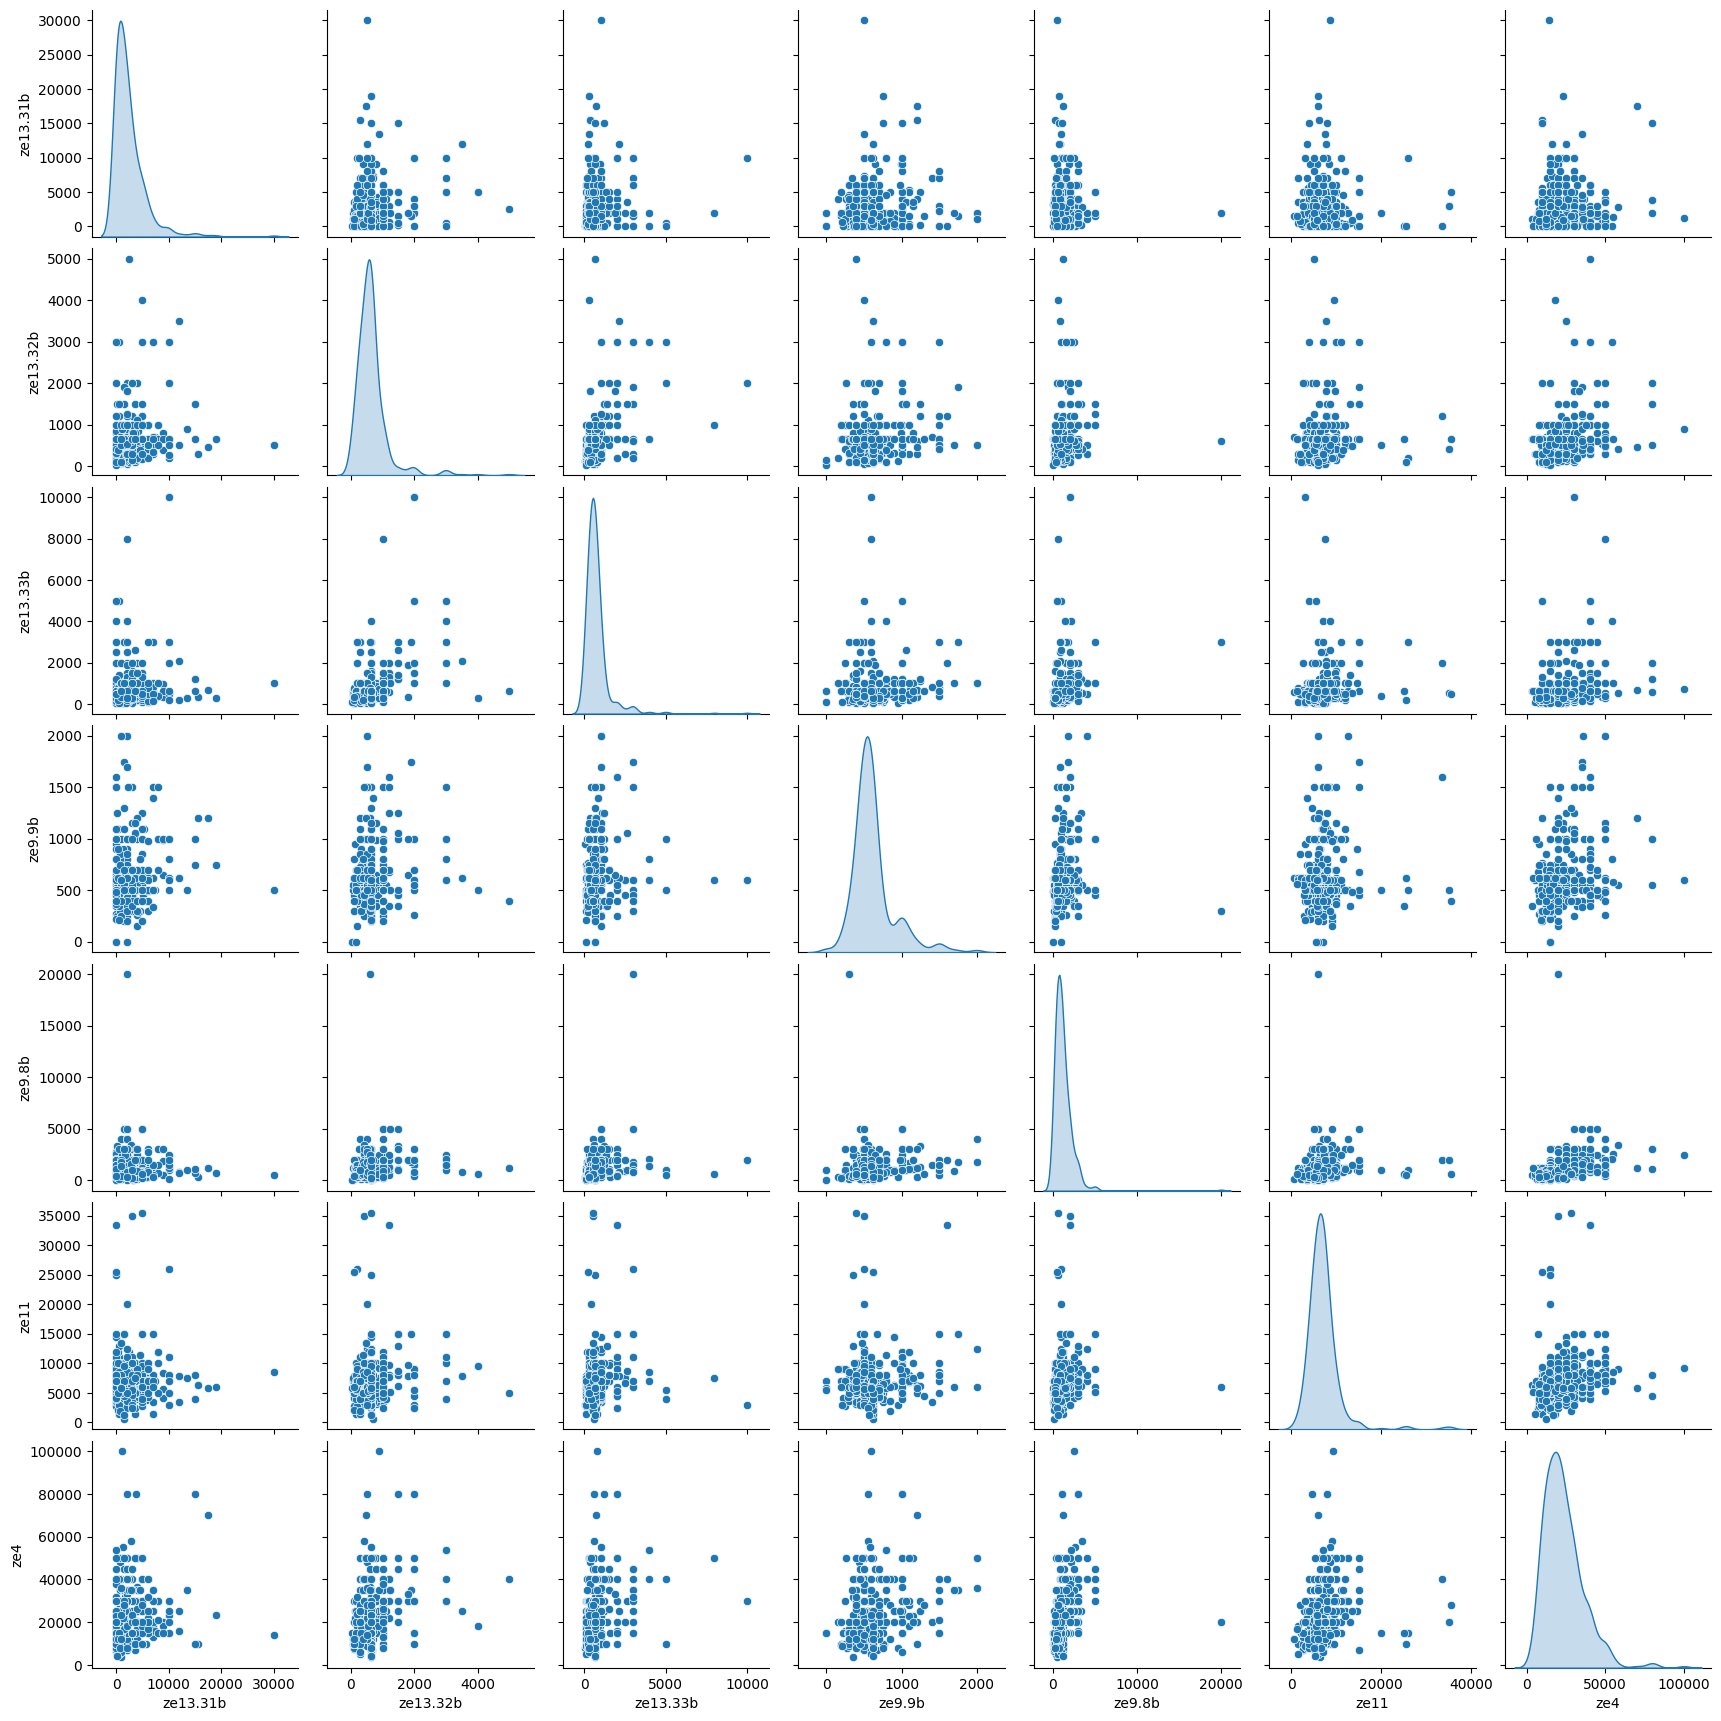
\includegraphics[scale=0.35]{./imgs/eda.png}
    \caption{Непараметрические распределения и диаграммы рассеивания для каждого из выбранных для факторного анализа признака}
\end{figure}   
\section{Метод главных компонент. Ортогональный базис. Снижение размерности.}

Поиск главных компонент с помощью SVD разложения. Для получения $n$-главных компонент необходимо взять первые $n$ сингулярных векторов, соответствующих $n$ сингулярным значениям в отсортированном по убыванию порядке. 
\[
  A = U\Sigma V^T
\]
где $U$ и $V$ -- ортогональные матрциы с ортонормированными собственными векторами матриц $AA^T$ и $A^TA$, соответственно. $\Sigma$ -- матрица сингулярных значений, каждое из которых равно квадратному корню собственного значения любой из матриц  $AA^T$ или $A^TA$ (собственные значения их равны).
\par В силу того, что изначальные данные обладали высокой дисперсией, они были прошкалированы (Standard Scaler). После чего был применен метод главных компонент. В результате были выбраны 4 компоненты, сохраняющие немногим более $78\%$ дисперсии.
\begin{figure}[H]
  \centering
  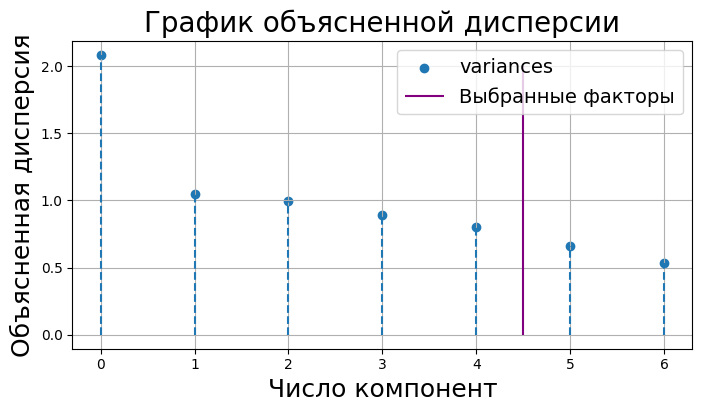
\includegraphics[scale=0.4]{./imgs/explained_var.png}
\end{figure}
Ниже представлен график собственных значений:
\begin{figure}[H]
  \centering
  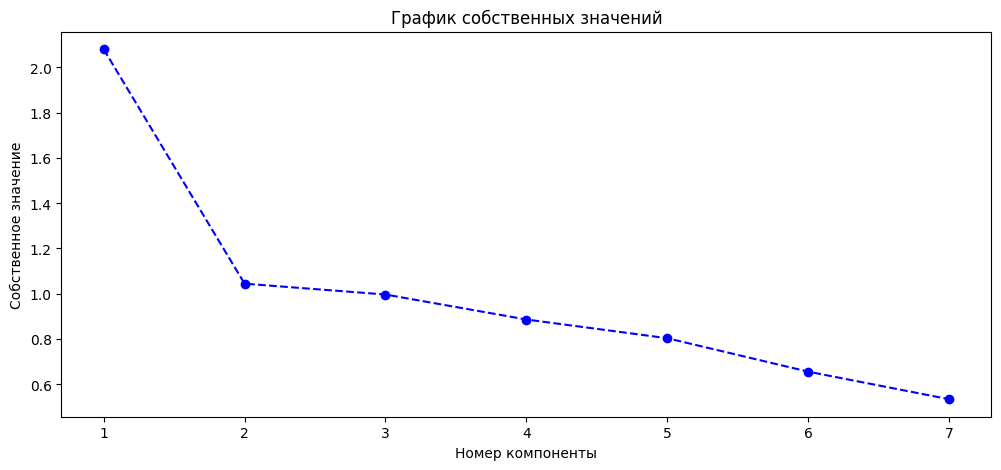
\includegraphics[scale=0.5]{./imgs/eigen_values.png}  
\end{figure}
Посмотрим на матрицу факторных нагрузок:
\begin{table}[H]
  \centering
  \begin{tabular}{|l|l|l|l|l|}
  \hline
  \backslashbox{Признак}{Номер компоненты}  &
    Factor 1 &
    Factor 2 &
    Factor 3 &
    Factor 4 \\ \hline
  Траты на медикаменты &
    0.141197 &
    -0.008138 &
    0.135708 &
    0.00865 \\ \hline
  Траты на моющие средства &
    \cellcolor[HTML]{9AFF99}0.575594 &
    0.106344 &
    0.043137 &
    \cellcolor[HTML]{9AFF99}0.197001 \\ \hline
  Траты на средства личной гигиены &
    \cellcolor[HTML]{9AFF99}0.687187 &
    0.269792 &
    0.043559 &
    -0.0059069 \\ \hline
  Траты на Интернет &
    0.029865 &
    0.243704 &
    \cellcolor[HTML]{9AFF99}0.640133 &
    -0.0019427 \\ \hline
  Траты на мобильную связь &
    0.113735 &
    \cellcolor[HTML]{9AFF99}0.493452 &
    \cellcolor[HTML]{FFFFFF}0.199075 &
    0.018566 \\ \hline
  \begin{tabular}[c]{@{}l@{}}Траты на квартиру\\ (аренда, коммунальные услуги)\end{tabular} &
    0.077945 &
    0.223865 &
    \cellcolor[HTML]{9AFF99}0.220932 &
    0.054067 \\ \hline
  \begin{tabular}[c]{@{}l@{}}Траты на питание\\ (дома и вне дома)\end{tabular} &
    0.150570 &
    \cellcolor[HTML]{9AFF99}0.627606 &
    0.106392 &
    \cellcolor[HTML]{9AFF99}0.589123 \\ \hline
  \end{tabular}
  \end{table}

  Попробуем интерпретировать компоненты:
  \begin{itemize}
    \item Первая компонента может показывать траты на предметы первой необходимости для домохозяйств;
    \item Вторая компонента в некой степени описывает ежемесячные траты;
    \item Третья компонента показывает траты на квартиру;
    \item Четвертую компоненту интерпретировать сложнее, можно попробовать как траты на питание и всё, что с этим связано (мытье посуды, например).
  \end{itemize}
  В силу того, что новое пространство сохраняет немалый процент дисперсии -- можно говорить о том, что снижение размерности позволительно. Посмотрим на данные после снижения размерности (в рамках двух первых компонент):
  \begin{figure}[H]
    \centering
    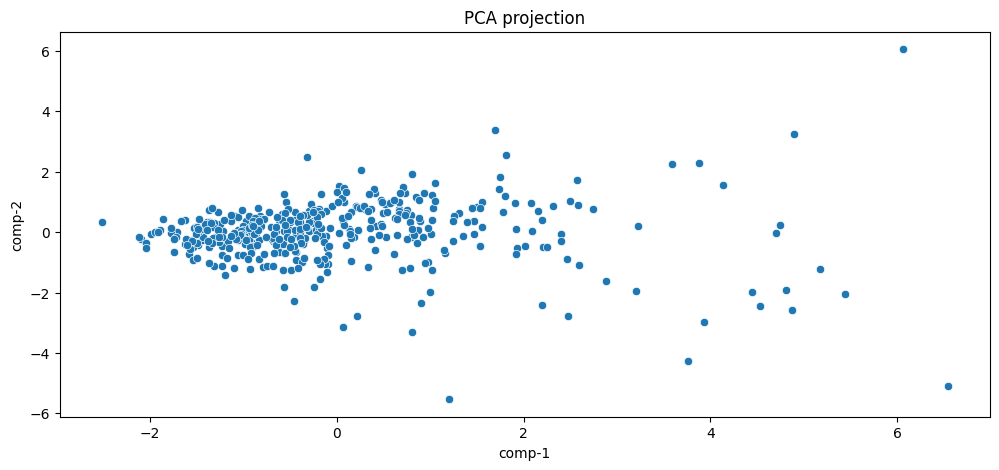
\includegraphics[scale=0.38]{./imgs/pca1.png}
  \end{figure}
\section{Расщепление смеси вероятностных распределений}
Для параметрической классификации был выбран признак логарифма денежного дохода. Построим непараметрическое эмпирическое распределение и непараметрическое распределение с ядерной оценкой плотности вероятности:
\begin{figure}[H]
  \centering
  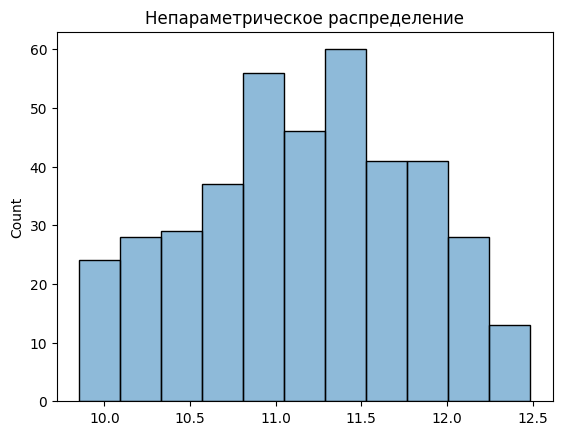
\includegraphics[scale=0.5]{./imgs/hist.png} \hspace*{0.5cm} 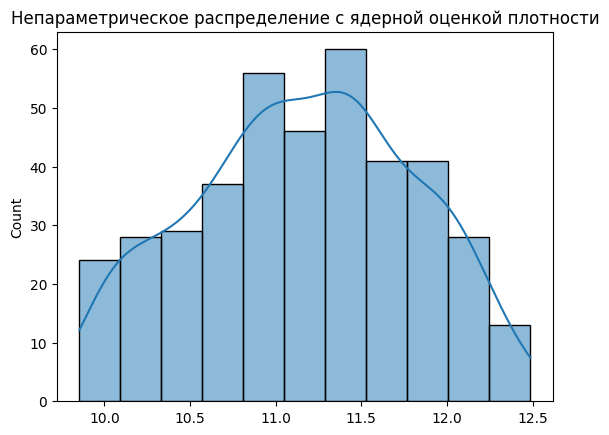
\includegraphics[scale=0.5]{./imgs/hist_kde.png}
\end{figure}
Здесь возможно композиция сразу нескольких распределений, попробуем композицию 3 колокообразных распределений. Воспользуемся EM-алгоритмом для нахождения весов и параметров распределения, чтобы представить искомое в виде их линейной комбинации вида: 
\[
    f(x) = \sum\limits_{j=1}^k q_j f(x, \theta_j).  
\]
Опишем модель. Одномерная модель (как в нашем случае) представляет собой следующее расщепление плотности:
\[
    p(x) = \sum\limits_{i=1}^K q_i f(x| \mu_i, \sigma_i).
\]
Причем
\[
    \sum\limits_{i=1}^K q_i = 1.
\]
Для многомерного случая:
\[
    p(\vec{x}) = \sum\limits_{i=1}^K q_i f(\vec{x}| \mu_i, \Sigma_i)
\]
\[
    f(\vec{x}| \mu_i, \Sigma_i) = \dfrac{1}{\sqrt{(2\pi)^K |\Sigma_i|}} \exp\left(-0.5(\vec{x} - \mu_i)^T \Sigma^{-1}_i (\vec{x} - \mu_i)\right)
\]
Как уже было сказано, для такого обучения без прецедентов используется $EM$-алгоритм, состоящий из нескольких шагов:
\begin{itemize}
  \item Инициализация:
  \begin{itemize}
    \item Случайно выбрать примеры без замены из датасета $X = \left\{x_1, \ldots, x_N\right\}$ и присвоить их значения оценкам средних $\{\hat{\mu}_i\}, \forall i = [1, \ldots, K]$;
    \item Для всех оценок дисперсии присвоить значение выборочной дисперсии:
    \[
      \hat{\sigma}_1^2,\ldots, \hat{\sigma}_K^2=\frac{1}{N}\sum_{i=1}^N (x_i - \overline{x})^2,
    \]
    где среднее -- выборочное среднее:
    \[
        \overline{x} = \dfrac{1}{N} \sum\limits_{i=1}^N x_i.
    \]
    \item Пропорции распределений оценить равномерным распределением:
    \[
        \hat{q}_1, \ldots, \hat{q}_2 = \dfrac{1}{K}.
    \]
  \end{itemize}
  \item Expectation (E) шаг:
  $\forall  i, k$ оценить вероятность, что $i$-ый сэмпл сгенерирован из $k$-ой компоненты:
  \[
    \hat{\gamma}_{ik} = p(C_k | x_i, \hat{q}, \hat{\mu}, \hat{\sigma}) = \dfrac{\hat{q}_k f(x_i | \hat{\mu}_k, \hat{\sigma}_k)}{\sum\limits_{j=1}^K \hat{q}_j f(x_i | \hat{\mu}_j, \hat{\sigma_j})}.
  \]
  \item Maximization (M) шаг:
  Пересчитать оценки в соответствии с посчитанными вероятностями принадлежности сэмплов к классам (компонентам, кластерам):
  \[
      \forall k: \hspace*{0.5cm} \begin{array}{c}
        \hat{q}_k = \sum\limits_{i=1}^N \dfrac{\hat{\gamma}_{ik}}{N}; \hspace*{1cm}
        \hat{\mu}_k = \dfrac{\sum\limits_{i=1}^N \hat{\gamma}_{ik}x_i}{\sum\limits_{i=1}^N \hat{\gamma}_{ik}} \\[0.5cm]
        \hat{\sigma}^2_k = \dfrac{\sum\limits_{i=1}^N \hat{\gamma}_{ik}(x_i - \hat{\mu}_k)^2}{\sum\limits_{i=1}^N \hat{\gamma_{ik}}}.
      \end{array}    
  \]
\end{itemize}
В итоге, получаем: 
\begin{figure}[H]
  \centering
  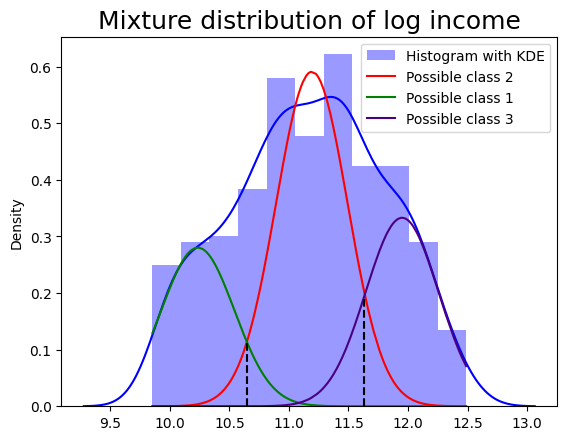
\includegraphics[scale=0.6]{./imgs/mix_logincome.png}
\end{figure}
Имеем три класса и границы их отделимости. Далее была произведена разметка выборки в соотвествии с полученными классами, чтобы сравнивать результаты с методами кластеризации и последующими регрессионными моделями.
\section{Кластеризация. KMeans, Hierarchiral, Spectral}
Для сравнения кластеризация производилась с помощью методом К средних, иерархической и спектральной кластеризаций. Для кластеризации по признаку логарифма дохода результаты схожи с расщеплением распределений и приведены ниже:
\begin{figure}[H]
  \centering
  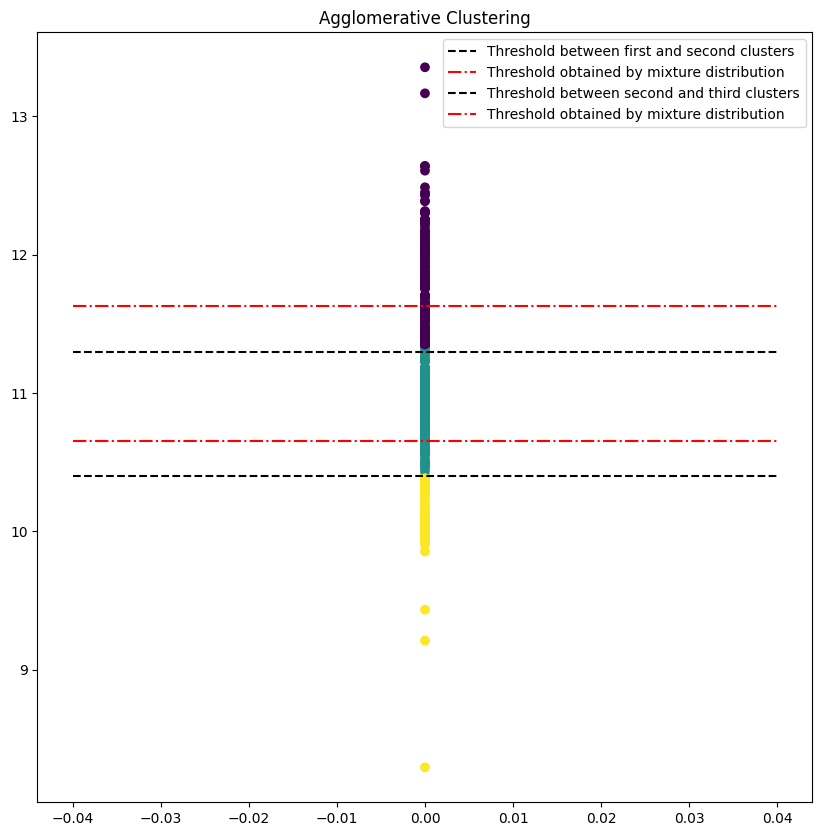
\includegraphics[scale=0.35]{./imgs/agglo.png} \hspace*{0.5cm} 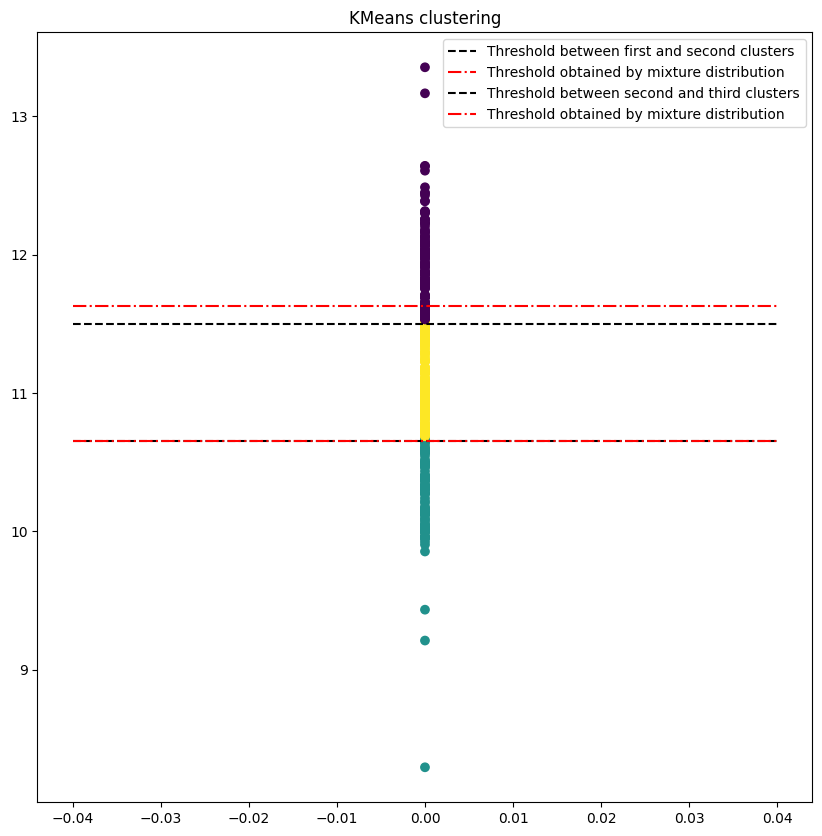
\includegraphics[scale=0.35]{./imgs/kmeans.png} \hspace*{0.5cm} 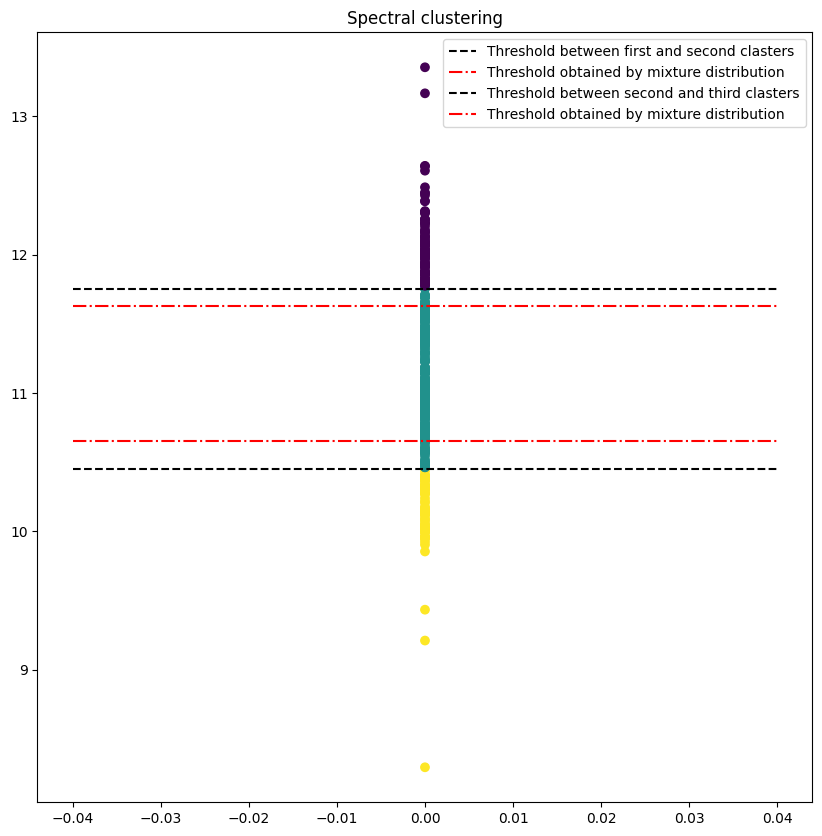
\includegraphics[scale=0.35]{./imgs/spectral.png}
\end{figure}
Дендрограмма для иерархической кластеризации представлена ниже:
\begin{figure}[H]
  \centering
  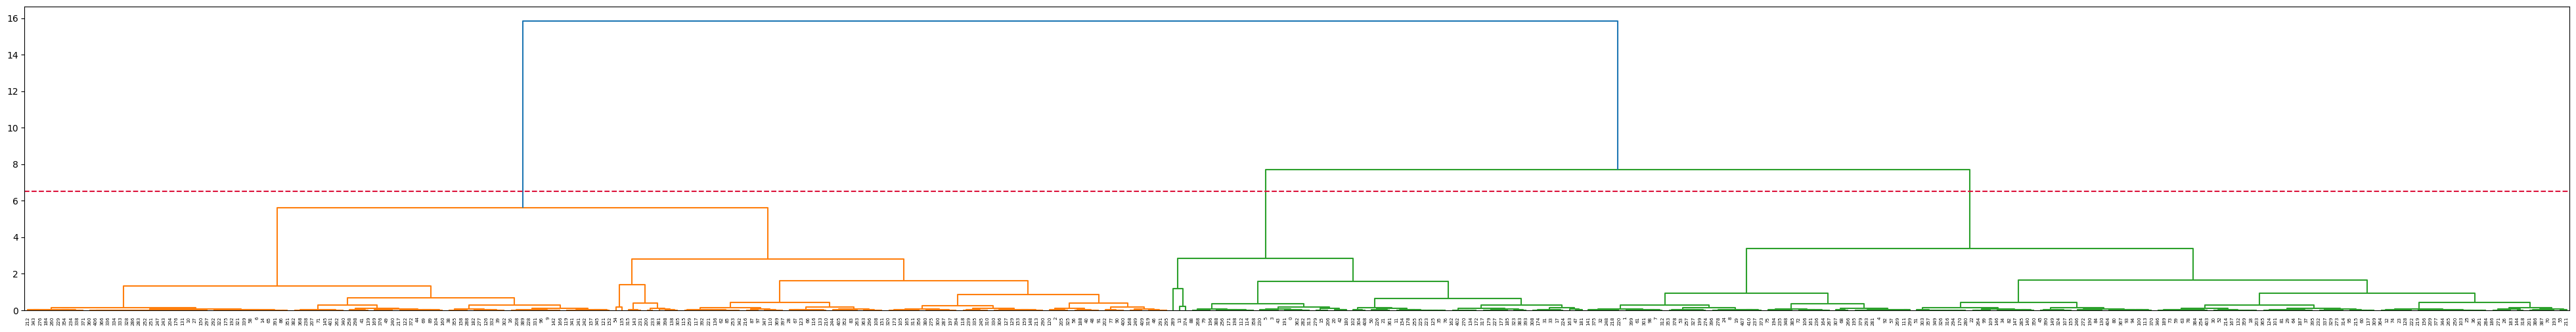
\includegraphics[scale=0.18]{./imgs/dendrogram.png}
\end{figure}
При кластеризации по объектам в пространстве главных компонентам присутствуют значительные отличия: 
\begin{figure}[H]
  \centering
  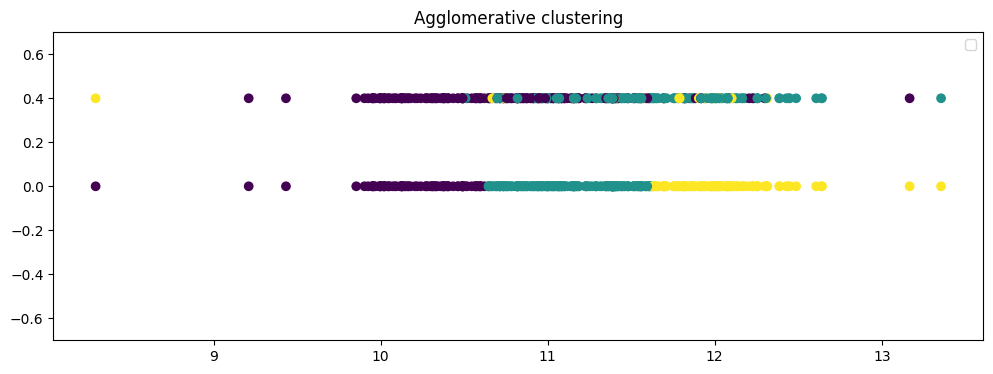
\includegraphics[scale=0.5]{./imgs/agglo_pca.png}
\end{figure}
\begin{figure}[H]
  \centering
  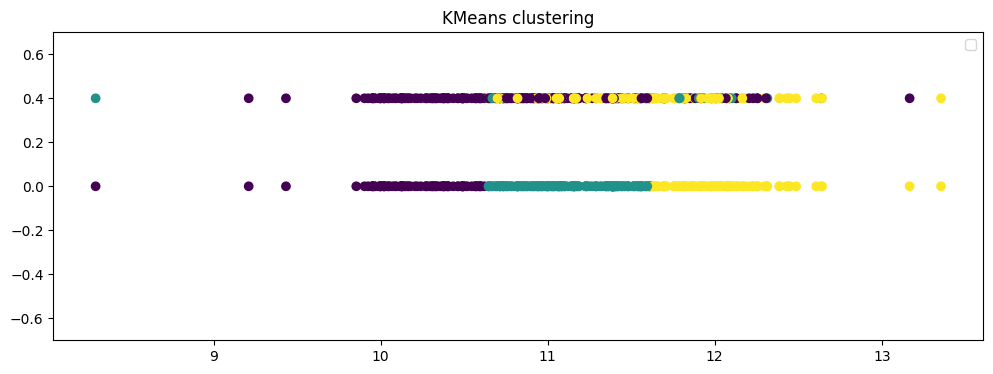
\includegraphics[scale=0.5]{./imgs/kmeans_pca.png}
\end{figure}
\begin{figure}[H]
  \centering
  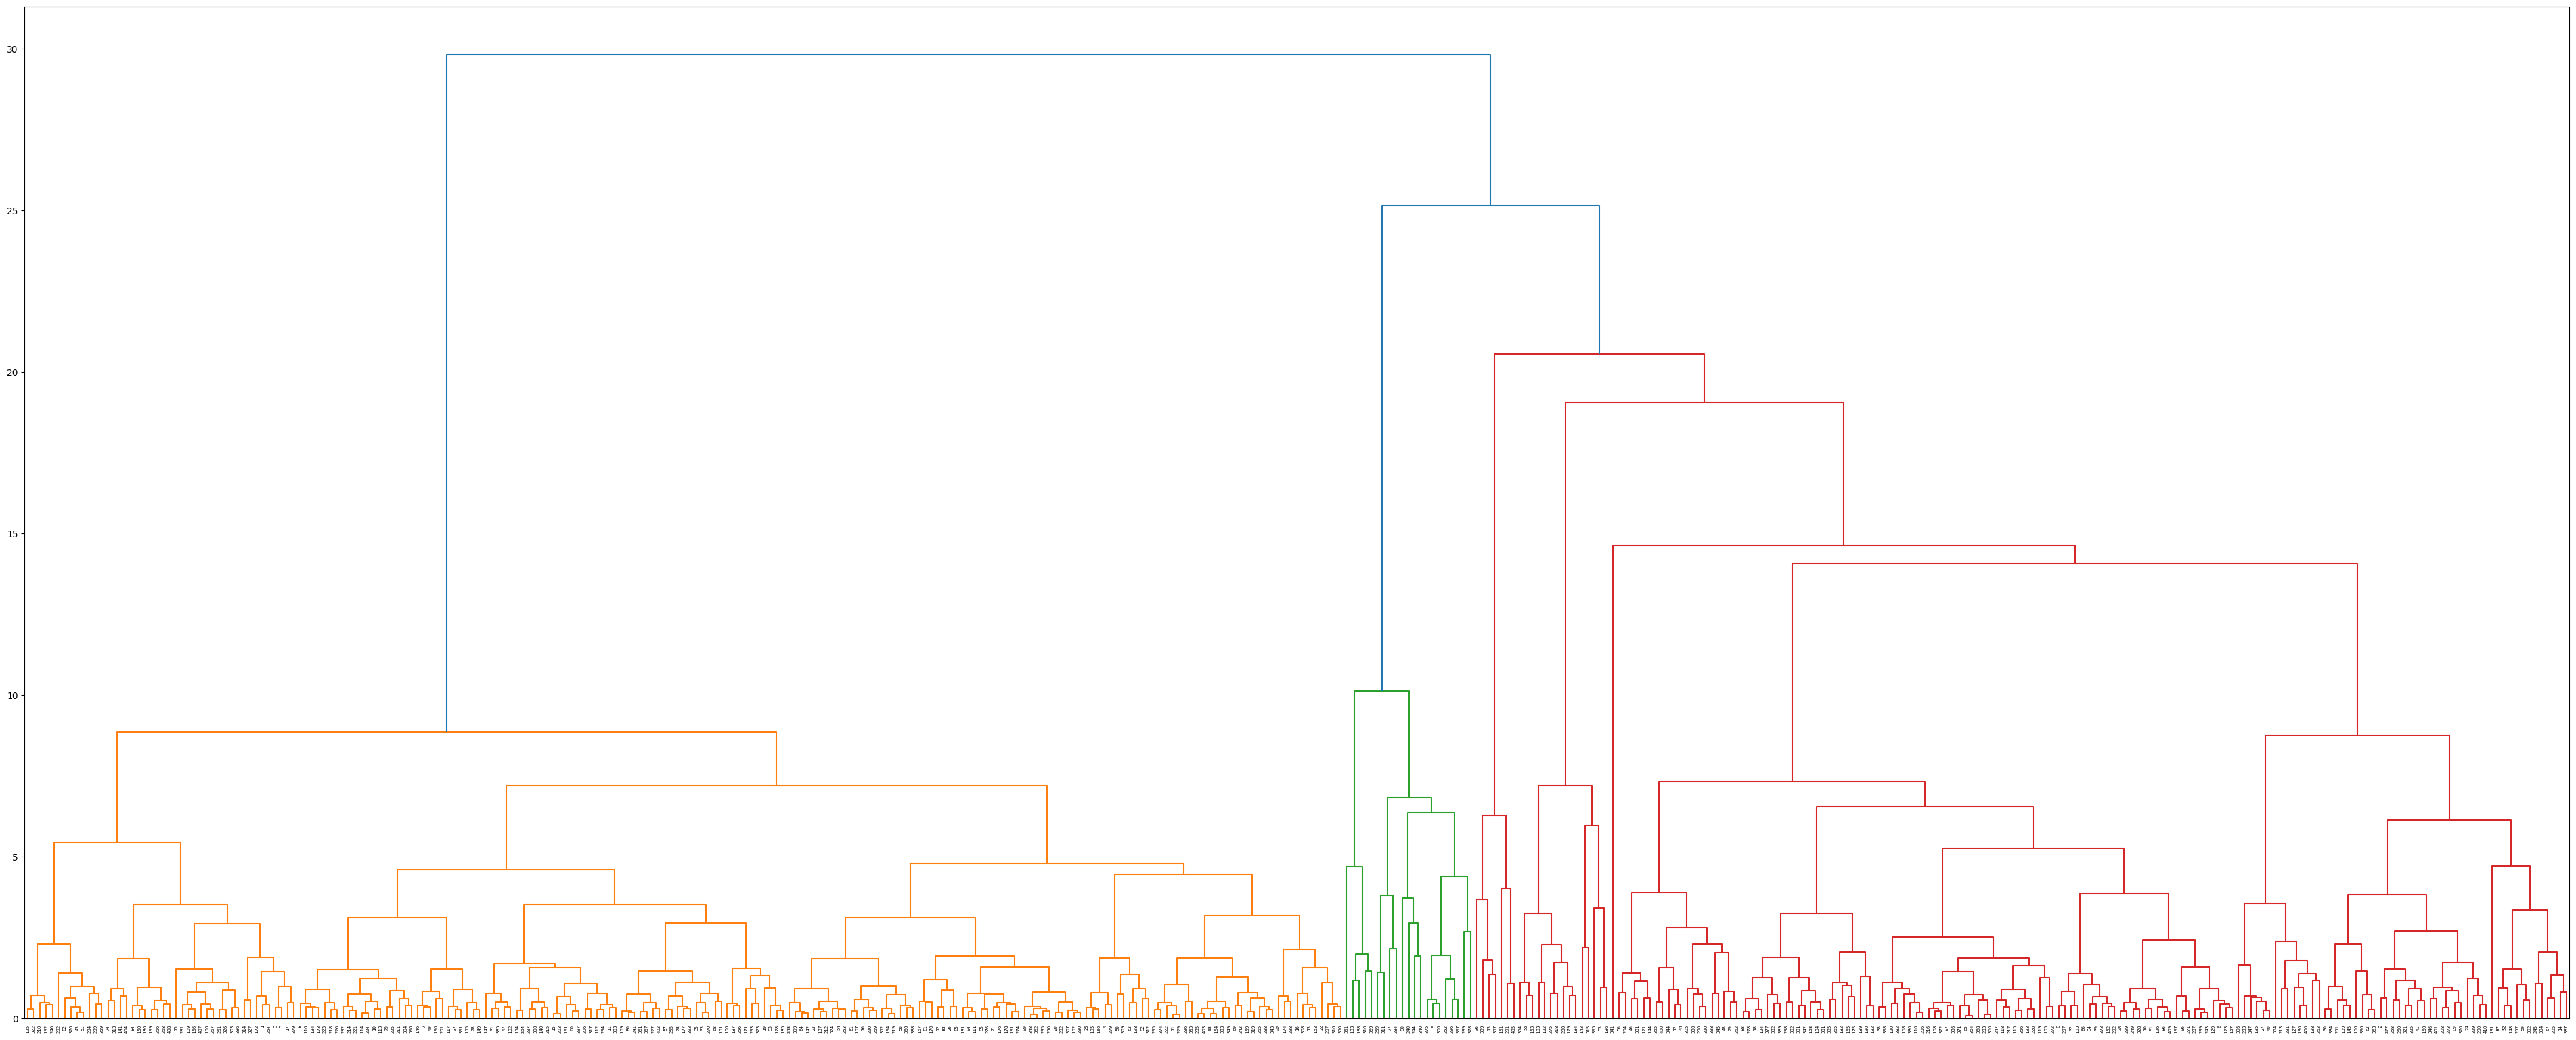
\includegraphics[scale=0.18]{./imgs/dendrogram_pca.png}
\end{figure}
Однако визуализация в рамках двух главных компонент, показывает о наличии структуры и валидности таких разбиений на кластеры:
\begin{figure}[H]
  \centering
  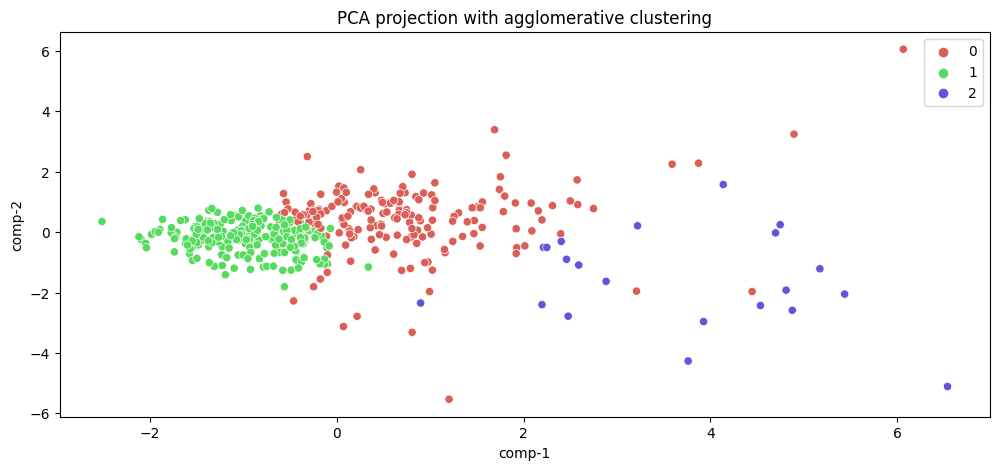
\includegraphics[scale=0.5]{./imgs/agglo_clusters.png}
\end{figure} 
\begin{figure}[H]
  \centering
  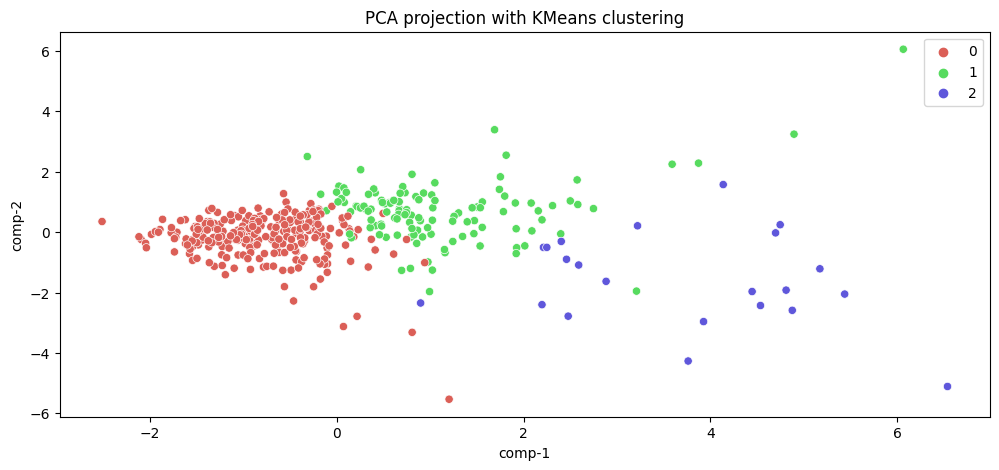
\includegraphics[scale=0.5]{./imgs/KMeans_clusters.png}
\end{figure} 
Конечно, в случае с расщеплением распределения денежных доходов всё не так хорошо, но он явно и не содержался в выбранных признаках для факторного анализа. Наличие, даже приведенной ниже структуры, уже говорит о ее существовании.
\begin{figure}[H]
  \centering
  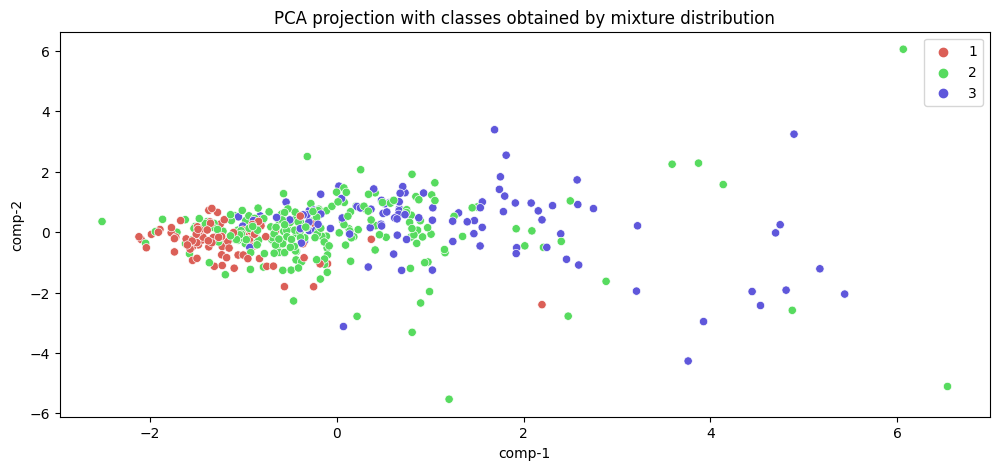
\includegraphics[scale=0.5]{./imgs/pca_classes.png}
\end{figure} 
\section{Классификация методом дискриминантного анализа}
Так же разметим выборки в соответствии с остальными методами кластеризации. Построим кросс-валидацию двумя методами: LeaveOneOut и стандартный KFoldation. Посмотрим на метрики точность и F1 меру (weighted обобщенную на многоклассовую классификацию).
\begin{table}[H]
  \centering
  \begin{tabular}{|c|cc|cc|}
  \hline
  \multirow{3}{*}{\backslashbox{Метрика}{Таргет}}                   & \multicolumn{2}{c|}{\multirow{2}{*}{income}} & \multicolumn{2}{c|}{pca\_cols}      \\ \cline{4-5} 
   & \multicolumn{2}{c|}{}                 & \multicolumn{1}{c|}{Hierarchical} & KMeans     \\ \cline{2-5} 
   & \multicolumn{1}{c|}{LOO} & KFoldation & \multicolumn{1}{c|}{LOO}          & KFoldation \\ \hline
  \multicolumn{1}{|l|}{accuracy}      & \multicolumn{1}{c|}{0.98}      & 0.9878      & \multicolumn{1}{c|}{0.898} & 0.893  \\ \hline
  \multicolumn{1}{|l|}{f1 (weighted)} & \multicolumn{1}{c|}{0.98}      & 0.9876      & \multicolumn{1}{c|}{0.898} & 0.8884 \\ \hline
  \end{tabular}
  \end{table}

  \begin{figure}[H]
    \centering
    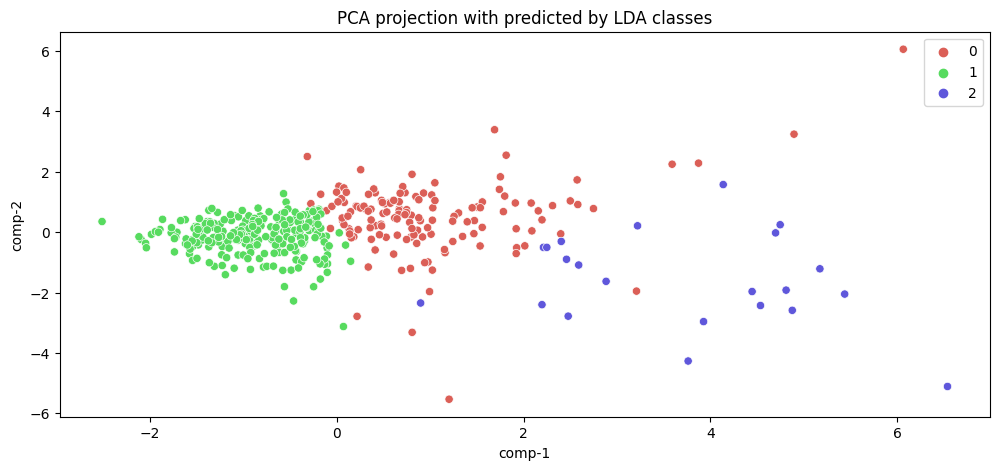
\includegraphics[scale=0.5]{./imgs/lda_clusters.png}
  \end{figure}
  \begin{figure}[H]
    \centering
    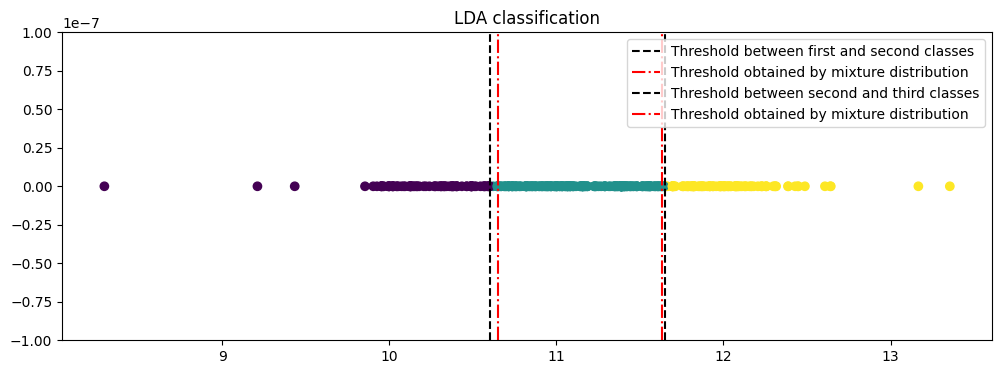
\includegraphics[scale=0.5]{./imgs/lda_income.png}
  \end{figure}
\section{Регрессионные модели}
Выбранные признаки для регрессии:
\begin{table}[H]
  \centering
  \begin{tabular}{|l|l|l|}
    \hline
    \multicolumn{1}{|c|}{Столбец} &
      Обозначение &
      \multicolumn{1}{c|}{Описание} \\ \hline
    zc1.1 &
      $x_1$ &
      \begin{tabular}[c]{@{}l@{}}Какова сегодня приблизительно рыночная стоимость такого \\ жилья, как Ваше?\end{tabular} \\ \hline
    zb1.o &
      $x_2$ &
      Сколько человек, включая Вас, в Вашей семье, домохозяйстве? \\ \hline
    zc6 &
      $x_3$ &
      \begin{tabular}[c]{@{}l@{}}Какова общая полезная площадь жилья у Вашей семьи, \\ то есть сумма площадей жилых комнат, кухни, ванной, туалета, \\ прихожей, кладовых и тому подобного в квартире (доме)?\end{tabular} \\ \hline
    zc5 &
      $x_4$ &
      \begin{tabular}[c]{@{}l@{}}Какую жилую площадь занимает Ваша семья? \\ Сколько квадратных метров составляет площадь \\ только жилых комнат?\end{tabular} \\ \hline
    zf12\_a &
      $x_5$ &
      \begin{tabular}[c]{@{}l@{}}Если все члены Вашей семьи лишатся всех источников дохода, \\ как долго Ваша семья сможет материально жить так же, как сейчас, \\ т.е. не уменьшая расходов, только за счет денежных сбережений, \\ ничего не продавая из имущества?\end{tabular} \\ \hline
    \end{tabular}
  \end{table}
  Последний признак является категориальным, обработка была сделана двумя способами (OneHotEncoding и LabelEncoder). Регрессия была построена с таргетом $y$ на логарифм дохода, точность была посчитана с помощью метрик R2, MSE и MAE. Результаты приведены ниже. После этого в соответствии с границами из расщепления распределений, был произведен перевод в кластеры и посчитаны метрики f1 и точность. После всего этого, была запущена кросс-валидация, и проверены остатки регрессии на гомоскедастичность (устойчивость дисперсии) и на нормальность распределения на каждом фолде кросс-валидации. В результате отклоняем гипотезу о нормальности распределения регрессионных остатков, но не отвергаем гипотезу о гомоскедастичности. Модель устойчива, но таргет не способен был полностью объяснен выбранными признаками. 
  \[
    \hat{y} = 0.00000029 x_1 + 0.3 x_2 - 0.00032x_3 + 0.0031 x_4 + 0.031 x_5 + 10.2. \hspace*{0.5cm} R2 = 0.344, \ MAE = 0.4018, \ MSE = 0.27.
  \]
  После перевода в классы:
  \[
      \text{accuracy score: } 0.6, \hspace*{0.5cm} \text{f\_1 score: } 0.634 
  \]
  Регрессионные остатки:
  \begin{figure}[H]
    \centering
    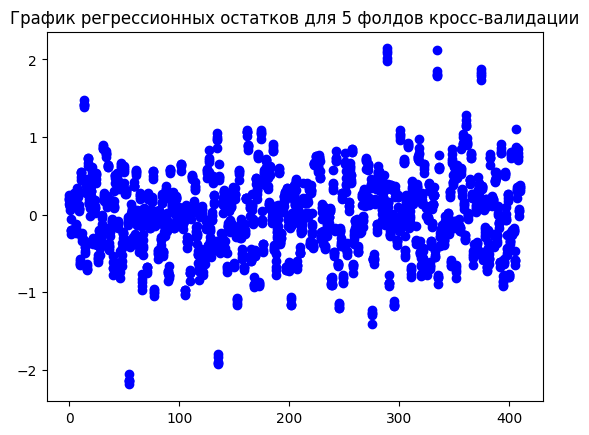
\includegraphics[scale=0.5]{./imgs/despendency.png}
  \end{figure}
  Гомоскедастичность с помощью теста Левена не отвергается. $p$-value велик. По критериям Шапиро-Уилка и теста Харке-Бера распределение остатков регрессии не нормально ($p$-value сильно близок к нулю).
\end{document}
